\section{Remarks}


\parbf{On graph comparison.}
Analogously to the tree comparison one can define \emph{graph comparison} for any graph by stating that there is a model configuration in $\HH$ such that 
\begin{itemize}
\item the distance between each pair of adjacent points is at most as big 
and
\item the distance between each pair of nonadjacent is at least as big.
\end{itemize}

\begin{thm}{Exercise}
Show that if a graph is a tree, then the graph comparison defined above is equivalent to the tree comparison defined at the beginning of the paper.
\end{thm}


Note that nonnegative and nonpositive curvature can be defined using the comparison for following two graphs on 4 vertexes:

\begin{center}
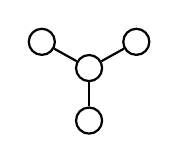
\begin{tikzpicture}[scale=1,
  thick,main node/.style={circle,draw,font=\sffamily\bfseries,minimum size=3mm}]

  \node[main node] (0) at (0,0) {};
  \node[main node] (1) at (-3/5,1/3){};
  \node[main node] (2) at (3/5,1/3){};
  \node[main node] (3) at (0,-2/3) {};

  \path[every node/.style={font=\sffamily\small}]
   (0) edge node[above]{}(1)
   (0) edge node[above]{}(2)
   (0) edge node[above]{}(3);
\end{tikzpicture}
\hskip30mm
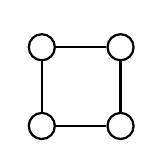
\begin{tikzpicture}[scale=1,
  thick,main node/.style={circle,draw,font=\sffamily\bfseries,minimum size=3mm}]

  \node[main node] (1) at (0,0) {};
  \node[main node] (2) at (0,1){};
  \node[main node] (3) at (1,1){};
  \node[main node] (4) at (1,0) {};

  \path[every node/.style={font=\sffamily\small}]
   (1) edge node[above]{}(2)
   (1) edge node[above]{}(4)
   (2) edge node[above]{}(3)
   (3) edge node[above]{}(4);
\end{tikzpicture}
\end{center}
If a graph $G$ has two induced subgraphs that isomorphic to each of these two graphs, then the corresponding graph comparison implies that the curvature vanish in the sense of Alexandrov.
In particular, any complete length spaces satisfying $G$-graph comparison is isometric to a convex set in a Hilbert space. 

By Reshetnyak majorization theorem,
the nonpositive curvature could be also defined using the comparison for cycle;
for example the 6-cycle --- the first graph the following diagram.

\begin{center}
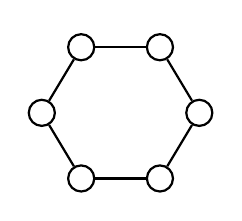
\begin{tikzpicture}[scale=1,
  thick,main node/.style={circle,draw,font=\sffamily\bfseries,minimum size=3mm}]

  \node[main node] (4) at (3/2,5/6){};
   \node[main node] (1) at (1/2,-5/6){};
  \node[main node] (2) at (3/2,-5/6){};
  \node[main node] (0) at (0,0){};
  \node[main node] (5) at (1/2,5/6){};
  \node[main node] (3) at (2,0){};


  \path[every node/.style={font=\sffamily\small}]
    (0) edge node[above]{}(1)
   (1) edge node[above]{}(2)
    (2) edge node[above]{}(3)
   (3) edge node[above]{}(4)
   (4) edge node[above]{}(5)
   (5) edge node[above]{}(0);
\end{tikzpicture}
\hskip30mm
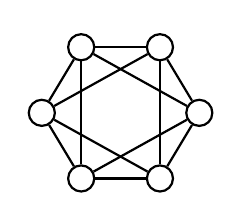
\begin{tikzpicture}[scale=1,
  thick,main node/.style={circle,draw,font=\sffamily\bfseries,minimum size=3mm}]

  \node[main node] (4) at (3/2,5/6){};
   \node[main node] (1) at (1/2,-5/6){};
  \node[main node] (2) at (3/2,-5/6){};
  \node[main node] (0) at (0,0){};
  \node[main node] (5) at (1/2,5/6){};
  \node[main node] (3) at (2,0){};


  \path[every node/.style={font=\sffamily\small}]
    (0) edge node[above]{}(1)
   (1) edge node[above]{}(2)
    (2) edge node[above]{}(3)
   (3) edge node[above]{}(4)
   (4) edge node[above]{}(5)
   (5) edge node[above]{}(0)
    (0) edge node[above]{}(2)
   (1) edge node[above]{}(3)
    (2) edge node[above]{}(4)
   (3) edge node[above]{}(5)
   (4) edge node[above]{}(0)
   (5) edge node[above]{}(1);
\end{tikzpicture}
\end{center}

The comparison for the octahedron graph (the second graph on the diagram) implies that the space is nonpositively curved.
The latter follows since in this graph, a 4-cycle appears as an induced subgraph.
On the other hand, this comparison might be stronger and it might be interesting to understand.

The quotients of Hilbert space provide motivating examples to consider the tree comparison (see Theorem~\ref{thm:hilbert-quotient}).
Unfortunately we do not have such guiding examples in nonpositive curvature spaces --- we can only fumble around for something without light. 


\parbf{On colored graph comparison.}
It is also possible to use graph with $(\mp)$-colored edges and define comparison by model configuration such that the distances between vertexes adjacent by a $(-)$-edge does not get larger and by $(+)$-edge does not get smaller (no condition on the remaining pairs).

\begin{center}
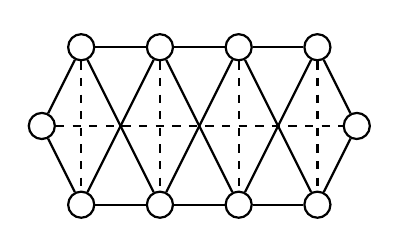
\begin{tikzpicture}[scale=1,
  thick,main node/.style={circle,draw,font=\sffamily\bfseries,minimum size=3mm}]

  \node[main node] (0) at (0.5,0){};
   \node[main node] (1) at (1,1){};
  \node[main node] (2) at (1,-1){};
  \node[main node] (3) at (2,1){};
  \node[main node] (4) at (2,-1){};
  \node[main node] (5) at (3,1){};
\node[main node] (6) at (3,-1){};
 \node[main node] (7) at (4,1){};
\node[main node] (8) at (4,-1){};
\node[main node] (100) at (4.5,0){};

  \path[every node/.style={font=\sffamily\small}]
    (0) edge[dashed] node[above]{}(100)
   (1) edge[dashed] node[above]{}(2)
    (3) edge[dashed] node[above]{}(4)
   (5) edge[dashed] node[above]{}(6)
   (7) edge[dashed] node[above]{}(8)
   (0) edge node[above]{}(1)
   (0) edge node[above]{}(2)
    (1) edge node[above]{}(3)
   (2) edge node[above]{}(4)
   (1) edge node[above]{}(4)
   (2) edge node[above]{}(3)
   (5) edge node[above]{}(3)
   (6) edge node[above]{}(4)
   (5) edge node[above]{}(4)
   (6) edge node[above]{}(3)
   (5) edge node[above]{}(7)
   (6) edge node[above]{}(8)
   (5) edge node[above]{}(8)
   (6) edge node[above]{}(7)
   (7) edge node[above]{}(100)
   (8) edge node[above]{}(100);
\end{tikzpicture}
\end{center}

For example, the $(2{\cdot}n+2)$-comparison (which holds in $\CAT[0]$ length spaces, see \cite{AKP}) can be considered as a comparison for the colored graph above, where $(-)$-edges are marked by solid lines and $(+)$-edges by dashed lines.


\parbf{Finite subsets of Alexandrov spaces.}
The following problem discussed in \cite[7.1]{AKP} was one of the original motivations to study the tree comparison:
\emph{Which finite metric spaces admit isometric embeddings into some Alexandrov spaces with nonnegative curvature.}


This problem is still open (as well as its analog for $\CAT(0)$ spaces).
According to \cite[4.1]{AKP}, the $(n-1)$-tree comparison provides a necessary condition for the problem $n$-point metric spaces.
An other well known necessary condition, the so called \emph{matrix inequality} turns out to be weaker than $(n-1)$-tree comparison; see the discussion below.
This condition is sufficient for the 4-point metric spaces.
It might be still sufficient for 5-point metric spaces,
but not for 6-point metric spaces.

The corresponding example of 6-point metric space was constructed by Sergei Ivanov, see \cite{AKP}.
Theorem~\ref{2(2)+3(1)}, provides a source for such examples --- any 6-point metric space that satisfy all 5-tree comparisons, but does not satisfy 2(2)-tree comparison provides an example.
This class of examples includes the example of Sergei Ivanov --- in the notations of \cite[7.1]{AKP} it does not satisfies the comparison for the tree $y/az(q/xb)$.

By Theorem~\ref{2(2)+3(1)} and a theorem in \cite{AKP}, 
5-tree and 2(2)-tree comparisons provide a necessary condition for 6-point metric spaces.
We expect that these conditions are sufficient

\begin{center}
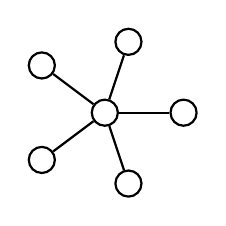
\begin{tikzpicture}[scale=1,
  thick,main node/.style={circle,draw,font=\sffamily\bfseries,minimum size=3mm}]

  \node[main node] (1) at (.3,-.9) {};
  \node[main node] (2) at (0,0){};
  \node[main node] (3) at (.3,.9){};
  \node[main node] (4) at (1,0) {};
  \node[main node] (5) at (-.8,-.6) {};
  \node[main node] (6) at (-.8,.6) {};

  \path[every node/.style={font=\sffamily\small}]
   (1) edge node[above]{}(2)
   (2) edge node[above]{}(3)
   (2) edge node[above]{}(4)
   (2) edge node[above]{}(5)
   (2) edge node[above]{}(6);
\end{tikzpicture}
\hskip30mm
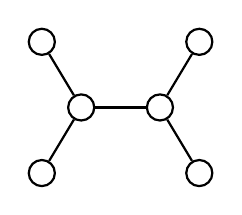
\begin{tikzpicture}[scale=1,
  thick,main node/.style={circle,draw,font=\sffamily\bfseries,minimum size=3mm}]

  \node[main node] (1) at (0,0) {};
  \node[main node] (2) at (1/2,5/6){};
  \node[main node] (3) at (0,10/6){};
  \node[main node] (4) at (2,0) {};
  \node[main node] (5) at (3/2,5/6) {};
  \node[main node] (6) at (2,10/6) {};

  \path[every node/.style={font=\sffamily\small}]
   (1) edge node[above]{}(2)
   (2) edge node[above]{}(3)
   (2) edge node[above]{}(5)
   (4) edge node[above]{}(5)
   (5) edge node[above]{}(6);
\end{tikzpicture}

\end{center}

Here an other candidate for a sufficient condition.

\begin{thm}{Question}\label{quest:all-tree}
Assume $F$ is a finite metric space that satisfies all tree comparisons.
Is it true that $F$ is isometric to a subset of an Alexandrov space with nonnegative curvature?
\end{thm}

Note that even for finite metric space the all tree comparison has to be checked for an infinite set of trees since one point of the space may be used as a label for several vertexes in the tree.

There is a chance that for 5-point and 6-point metric spaces, the condition in Question~\ref{quest:all-tree} is also necessary. 
However, since there are nonnegatively curved Riemannian manifolds that do not satisfy 4(1)-tree comparison, 
Theorem~\ref{thm:convexity} implies that this condition can not be necessary for 7-point metric spaces.

\medskip

For any metric space $X$ with an isometric group action $G\acts X$ with closed orbits the quotient map $X\to X/G$ is a submetry.
In particular, by Theorem~\ref{thm:hilbert-quotient}, if $G\acts \HH$ is an isometric action with closed orbits on the Hilbert space, then the quotient space $\HH/G$ satisfies all tree comparisons.

\begin{thm}{Question}
Assume $X$ is a metric space satisfying all tree comparisons.
Is it always possible to construct an isometric group action with closed orbits on the Hilbert space $G\acts \HH$ such that $X$ is isometric to a subset in $\HH/G$?
\end{thm}


\parbf{On matrix inequality.}
The comparison for monopolar trees has an algebraic corollary which was used Urs Lang and Viktor Schroeder in \cite{LS}, a similar inequality was used by Karl-Theodor  Sturm  in \cite{sturm}. 

Namely, given a point array $p,x_1,\dots,x_n$ in a metric space $X$ consider the $n{\times}n$-matrix $M$ with the components 
\[m_{i,j}=\tfrac12\cdot(|x_i-p|^2+|x_j-p|^2-|x_i-x_j|^2).\]
If the tree comparison for $p/x_1,\dots,x_n$ holds, then 
\[\bm{s}\cdot M\cdot \bm{s}^\top\ge 0\eqlbl{eq:sMs}\]
for any vector $\bm{s}=(s_1,\dots,s_n)$ with nonnegative components.

The converse does not hold; that is, for some point array $p,x_1,\dots,x_n$ in a metric space the inequality \ref{eq:sMs} might hold, while the tree comparison for $p/x_1x_2x_3x_4x_5$ does not.
(We do not know an explicit way to describe tree comparisons using a system of inequalities.)

\begin{wrapfigure}{r}{22 mm}
\vskip-0mm
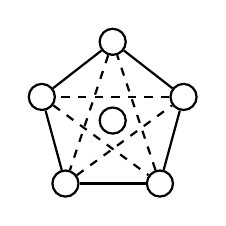
\begin{tikzpicture}[scale=1,
  thick,main node/.style={circle,draw,font=\sffamily\bfseries,minimum size=3mm}, ]

    \node[main node] (0) at (0,0){};
     \node[main node] (1) at (.6,-.8) {};
     \node[main node] (2) at (.9,.3){};
     \node[main node] (3) at (0,1) {};
  \node[main node] (4) at (-.9,.3) {};
  \node[main node] (5) at (-.6,-.8) {};

  \path[every node/.style={font=\sffamily\small}]
  (1) edge node[above]{}(2)
  (2) edge node[above]{}(3)
  (3) edge node[above]{}(4)
  (4) edge node[above]{}(5)
  (5) edge node[above]{}(1)
  (1) edge[dashed] node[above]{}(3)
  (2) edge[dashed] node[above]{}(4)
  (3) edge[dashed] node[above]{}(5)
  (4) edge[dashed] node[above]{}(1)
  (5) edge[dashed] node[above]{}(2);
\end{tikzpicture}
\end{wrapfigure}

An example can be constructed by perturbing the configuration on the plane as on the diagram ---
if the diameter of diagram is 1, 
then increasing the distances between the pairs of points connected by dashed lines by $\eps=10^{-9}$ and decreasing  the distances between the pairs of points connected by sold lines by $\delta=10^{-6}$ does the job.
The obtained metric 6-point metric space satisfies the matrix inequality with center at each point, but does not satisfy the tree comparison with the pole at the central point.

Many necessary conditions on finite subsets of nonnegatively curved Alexandrov spaces are known;
in addition to the comparisons discussed above, 
let us mention the authors results in \cite{lebedeva-petrunin} and \cite{petrunin}
and the Markov type inequality proved by Shin-ichi Ohta in \cite{ohta};
see also the survey by Assaf Naor \cite{naor} and the references there in.

\parbf{On tree comparisons in length spaces.}
Note that if a tree $T$ is not a path, then it contains a tripod as subtree.
Therefore $T$-tree comparison implies Alexandrov comparison, in particular any complete length-metric space satisfying $T$-tree comparison is a nonnegatively curved Alexandrov space.

It is straightforward to generalize Theorem~\ref{thm:3(1)+2(2)} to  Alexandrov spaces; that is, we have the following theorem.

\begin{thm}{Theorem}
A complete length space $L$ satisfies  3(1) or 2(2)-tree comparison if and only if $L$ is a nonnegatively curved Alexandrov space.
\end{thm}

We expect that Theorem~\ref{thm:convexity} (after appropriate reformulation) can be also generalized to Alexandrov spaces --- the only obstacle we see is the proof of Proposition~\ref{prop:CTIL}.
Such a generalization would characterize length-metric spaces satisfying most of 4(1)-tree comparison (as well as most of bipolar tree comparisons).

The Alexandrov spaces that satisfy 4(1) remind the quotients of Riemannian manifolds by isometric group actions. 
For example we expect that if a finite dimensional Alexandrov space $A$ satisfies 4(1)-tree, then the tangent space at any point $p\in A$ is a product of a Euclidean space $\mathbb{E}^k$ and a cone $K$ over space $\Sigma$ of diameter at most $\tfrac\pi2$ (the space $\Sigma$ might be empty, in this case $K$ is a one-point space).
In particular it implies that the set of all metric singularities of $A$ is an extremal subset, see \cite{perelman-petrunin}.
(For big branchy trees, the properties of spaces with the tree comparison should remind the quotients of Hilbert space even more.)

\parbf{On MTW.}
Recall that the condition (\textit{\ref{thm:convexity:MTW}}) in Theorem~\ref{thm:convexity} is named MTW$^{\not\perp}$.

Recall that for Riemannian manifolds, 3(1) and 2(2)-tree comparisons are equivalent to the nonnegative sectional curvature and 4(1) (as well as all $m$($n$)-tree comparison if $\max\{m,n\}\ge 4$) are equivalent to CTIL+MTW$^{\not\perp}$.
The meaning of tree comparisons for 3(2) and 3(3) remains unclear, one can only say that it is between Alexandrov comparison and CTIL+MTW$^{\not\perp}$.

\begin{thm}{Question}
What are the relations between 3(2) and 3(3)-tree comparisons,  MTW$^{\not\perp}$ and MTW for Riemannian manifolds with or without CTIL condition?
\end{thm}

For example, as we mentioned, MTW$^{\not\perp}$ is stronger than MTW, but we fail to show that it is strictly stronger.
In other words, we do not have an example of a (CTIL) Riemannian manifold that is MTW, but not MTW$^{\not\perp}$.
Another example: it might happen that 3(3)-tree comparison is equivalent to MTW+CTIL which would provide a synthetic description of these conditions.

We also do not know whether globalization theorem holds, for MTW$^{\not\perp}$ (or equivalently for 4(1)-tree comparison); in other words \emph{is it true that local MTW$^{\not\perp}$ implies gloabal MTW$^{\not\perp}$?}

The following two questions are well known for MTW;
partial answers are given in \cite{MTW+CTIL+} and \cite{loeper} correspondingly.
The question might be easier for MTW$^{\not\perp}$.

\begin{thm}{Question}
Is it true that MTW (or MTW$^{\not\perp}$) implies CTIL?
\end{thm}

Note that if the globalization holds for MTW$^{\not\perp}$, then by Theorem~\ref{thm:convexity}, MTW$^{\not\perp}$ implies CTIL.

\begin{thm}{Question}
Is it true that CTIL+MTW (or CTIL+MTW$^{\not\perp}$) on a compact Riemannian manifold implies TCP?
\end{thm}

By Theorem~\ref{thm:convexity}, CTIL+MTW$^{\not\perp}$ is equivalent to 4(1)-tree comparison. 
Therefore the MTW$^{\not\perp}$-vesion of the last question can be reformulated the following way:

\begin{thm}{Question} Is it true that 4(1)-tree comparison on a compact Riemannian manifold implies TCP?
\end{thm}

